\documentclass[10pt,sigconf]{acmart}
\settopmatter{printacmref=false} % Removes citation information below abstract
\renewcommand\footnotetextcopyrightpermission[1]{} % removes footnote with conference information in first column
\pagestyle{plain} % removes running headers
\setcopyright{none} % removes copyright information





\usepackage[utf8]{inputenc}
\usepackage{booktabs} % For formal tables
\usepackage{array}
\usepackage{commath}
\newcommand*\rotbf[1]{\rotatebox{90}{\textbf{#1}}}
\newcommand{\specialcell}[2][c]{\begin{tabular}[#1]{@{}l@{}}#2\end{tabular}}
\newcommand{\specialcellbold}[2][c]{%
  \bfseries
  \begin{tabular}[#1]{@{}l@{}}#2\end{tabular}%
}

% Copyright
%\setcopyright{none}
%\setcopyright{acmcopyright}
%\setcopyright{acmlicensed}
% \setcopyright{rightsretained}
%\setcopyright{usgov}
%\setcopyright{usgovmixed}
%\setcopyright{cagov}
%\setcopyright{cagovmixed}

\begin{document}
\title{Comment Volume Prediction}
\subtitle{Text Mining in Practice} % do we need that?

\author{Johannes M. Kroschewski}
\affiliation{%
	\institution{Hasso-Plattner-Institut,\\ University of Potsdam}
	\streetaddress{Prof.-Dr.-Helmert-Str. 2–3}
	\city{Potsdam} 
	\state{Germany} 
	\postcode{14482}
}
\email{johannes.kroschewski@student.hpi.de}

\author{Friedrich C. Schöne}
\affiliation{%
	\institution{Hasso-Plattner-Institut,\\ University of Potsdam}
	\streetaddress{Prof.-Dr.-Helmert-Str. 2–3}
	\city{Potsdam} 
	\state{Germany} 
	\postcode{14482}
}
\email{friedrich.schoene@student.hpi.de}

\author{Nils Straßenburg}
\affiliation{%
  	\institution{Hasso-Plattner-Institut,\\ University of Potsdam}
	\streetaddress{Prof.-Dr.-Helmert-Str. 2–3}
	\city{Potsdam} 
	\state{Germany} 
	\postcode{14482}
}
\email{nils.strassenburg@student.hpi.de}

% The default list of authors is too long for headers}
\renewcommand{\shortauthors}{M. Kroschewski et al.}


\begin{abstract}
	abstract text \footnote{abstract footnote}
\end{abstract}

\begin{CCSXML}
	% TODO
<ccs2012>
 <concept>
  <concept_id>10010520.10010553.10010562</concept_id>
  <concept_desc>Computer systems organization~Embedded systems</concept_desc>
  <concept_significance>500</concept_significance>
 </concept>
 <concept>
  <concept_id>10010520.10010575.10010755</concept_id>
  <concept_desc>Computer systems organization~Redundancy</concept_desc>
  <concept_significance>300</concept_significance>
 </concept>
 <concept>
  <concept_id>10010520.10010553.10010554</concept_id>
  <concept_desc>Computer systems organization~Robotics</concept_desc>
  <concept_significance>100</concept_significance>
 </concept>
 <concept>
  <concept_id>10003033.10003083.10003095</concept_id>
  <concept_desc>Networks~Network reliability</concept_desc>
  <concept_significance>100</concept_significance>
 </concept>
</ccs2012>  
\end{CCSXML}

\ccsdesc[500]{Computer systems organization~Embedded systems}
\ccsdesc[300]{Computer systems organization~Redundancy}
\ccsdesc{Computer systems organization~Robotics}
\ccsdesc[100]{Networks~Network reliability}

\keywords{text mining}

\maketitle

\section{Introduction}
In the last two decades, the possibilities of discussing news articles changed radically.
One of the most significant changes is that nowadays readers are able to share their opinion about a published article directly, e.g.\ in a comment section.
Despite the positive aspects of this freedom it is also often misused.
In consequence comment sections of online newspapers often get moderated which binds resources and is cost intensive.
In order to schedule publication times and plan moderator team sizes, it would be helpful to know which of the published articles will receive a large number of comments before their release.

Related work is trying to predict the comment volume of newspaper articles by using a random forest approach \cite{tsagkias2009predicting}.
Also using a random forest, Ambroselli et al.\ defined the classification task of identifying the weekly top $10\%$ of articles with the highest comment volume \cite{ambroselli2018prediction}.

In this study, we take the same classification task and explore whether a deep learning approach can outperform their model on a similar dataset.
We consider several different models and features which can be broken down into: (a) an analysis of the influence of different article features on the prediction performance, (b) the evaluation of different model architectures, and (c) a comparison of our results against other baselines.


\section{Dataset}
Our work is based on a dataset taken from the British newspaper \textit{The Guardian} that contains approximately $626$K article URLs with $61.5$M corresponding comments from $1.25$M authors. 
The comment data provided us with the comment text itself, the author, the timestamp when the comment was posted, a reference of the parent comment, and the number of upvotes. Additionally, we had the comment author's username and a dedicated reference. 

The comments were posted between 2006 and 2017. All $1.25$M users wrote at least one comment, $22$\% of them more than $10$, and $6$\% over $100$.
The given articles are published in one out of $79$ categories. In total, $18$\% of all released articles are published under the category \textit{comment is free} which is used to debate contentious issues. Consequently, this category is also the most commented one. 
Each of the others, e.g. \textit{sport}, \textit{music}, and \textit{politics} covers less than $7$\% in the given dataset.

The number of comments of past articles is essential to predict the comment volume of similar articles in the future. 
To decide if a given article was in the top $10$\% of the most commented articles within its released week could be determined by simply counting the corresponding comments of each article.
%The number of comments of a given article is essential to predict the comment volume of similar articles in the future. Fortunately, this could be determined by simply counting the corresponding comments of each article. Afterwards, we were able to decide if a given article was in the top $10$\% of the most commented articles within its released week.

\subsection{Data Cleaning}
Analysing the dataset, we noticed that the distribution of the number of comments exhibited a bizarre peak at exactly $50$ comments per article. Therefore, we did not take these articles into account which reduced our dataset about $2$\% of the given articles.

To avoid anomalies using features that we derived from the articles, e.g. the publication time, we removed a small amount of articles that were released on 29th of February.

\subsection{Data Enrichment}
To enrich our dataset, we used the offical \textit{Guardian API} to get the article text and further attributes like the category, the headline, and the publication time.
Due to API restrictions we were not able to download all articles which is why the amount of articles was reduced about $11$\%.
Furthermore, we extracted metadata like the headline and article word count, the time data describing the day of the week, the day of the year, the hour and the minute of the publication date.

We suppose that articles that are released at a similar time and discussing a related topic are likely to share the amount of comments. To take this behaviour into account, we've developed a \textit{competitive score} (\ref{eq:competitive_score}) as an additional feature.

\begin{equation} \label{eq:competitive_score}
	compet_i = \sum_{n=1}^{j} \frac{\sigma'(t_i - t_j)}{\norm{\overrightarrow{a_i} - \overrightarrow{{a_j}}}^2}, i \neq j
\end{equation}

\begin{flalign*}
	\sigma&: \text{sigmoid function} & \\
	t_i&: \text{publication date of article } i & \\
	\overrightarrow{a_i}&: \text{doc2vec vector of article } i \text{ text}& \\
\end{flalign*}

The numerical value of $compet_i$ describes how much a given article $i$ competes with all other articles. Thereby, the difference of the publication time of the given articles determines how close they are published to each other. For the calculation of this feature, we've considered all articles that were released within a timespan of $\pm3$h.
In pratice, articles will be often published at the same time which implies that the time difference can be zero. This is also a reason why we apply the derivate of the sigmoid function in the numerator.
To decide if articles are discussing a similar topic, we've trained the \textit{doc2vec} algorithm \cite{le2014doc2vec} on our article corpus and use the Euclidean distance to calculate how similar articles to each other are. We square the distance in the denominator to increase the impact of the article similarity.

In the following, we call the cleaned and enriched dataset the Guardian Article and Comment Corpus (GACC). Finally, the GACC contains approximately $547$K articles with $58.6$M comments.


\section{Methodology}
To evaluate the quality of our features, different architectures were implemented to compare how accurately they predict comment volume.
All seven architectural models use single or related features as input and generate a binary classification output using sigmoid as the activation function. 
Each model has an identifier which will be used as a reference within the further text.

\subsection{Architectures}

\paragraph{Model 1} 
Takes the article headline as input.
The headline length is normalized before embedding the words using an embedding layer which is initialized with pretrained glove embeddings \cite{pennington2014glove}.
The model uses a dense and a batch normalization layer as the hidden layers.

\paragraph{Model 2}
Takes the article headline as input which is than embedded as in \textit{Model 1}. 
A convolutional layer with kernel sizes one, three, and five is used instead of a dense layer as well as a pooling layer as proposed by Kim \cite{kim2014convolutional}.

\paragraph{Model 3} 
Takes the first $50$ words of the article text which are embedded the same way as in \textit{Model 1} and \textit{2}. However, the input is processed through an LSTM layer outputting its last cell state.

\paragraph{Model 4} 
Takes the article category as input.
The category reference gets embedded using an embedding layer and is processed through both a dense and a batch normalization layer.

\paragraph{Model 5} 
Takes temporal features of the article's publication date as input.
The features are minute, hour, day of the week, and day of the year.
They get processed the same way as in \textit{Model 4}.

\paragraph{Model 6} 
Takes the word counts from the headline and the article.
The logarithm is calculated for both of them and is used to create exponential sized bins for different lengths.
Each logarithm gets embedded and processed as in \textit{Model 5} and \textit{6}.

\paragraph{Model 7} 
Takes the competitive score as defined in \autoref{eq:competitive_score} and processes it through a dense layer as well as a batch normalization layer.

\subsection{Training}
The GACC was divided into training, validation, and test sets using a $0.70/0.15/0.15$  distribution with respect to the time of publication.

Due to the strongly imbalanced class sizes of the training set, we use class weights to penalise our models in case of a wrong classification.
During the training, they influence the weighting of the loss indirectly proportional to the class size of a giving training sample.

\subsection{Combined Architectures}
We combined several models to explore how using multiple features simultaneously would impact our results.
These combined models share the classification layers but not the hidden layers.
Specific models were only combined if they performed adequately and if their results had some correlation.
Combining these two metrics, we had a large set of models we were able to choose from.
The correlations between each model pair are shown in Figure \ref{fig:correlation_matrix}. 

\begin{figure}[h]
	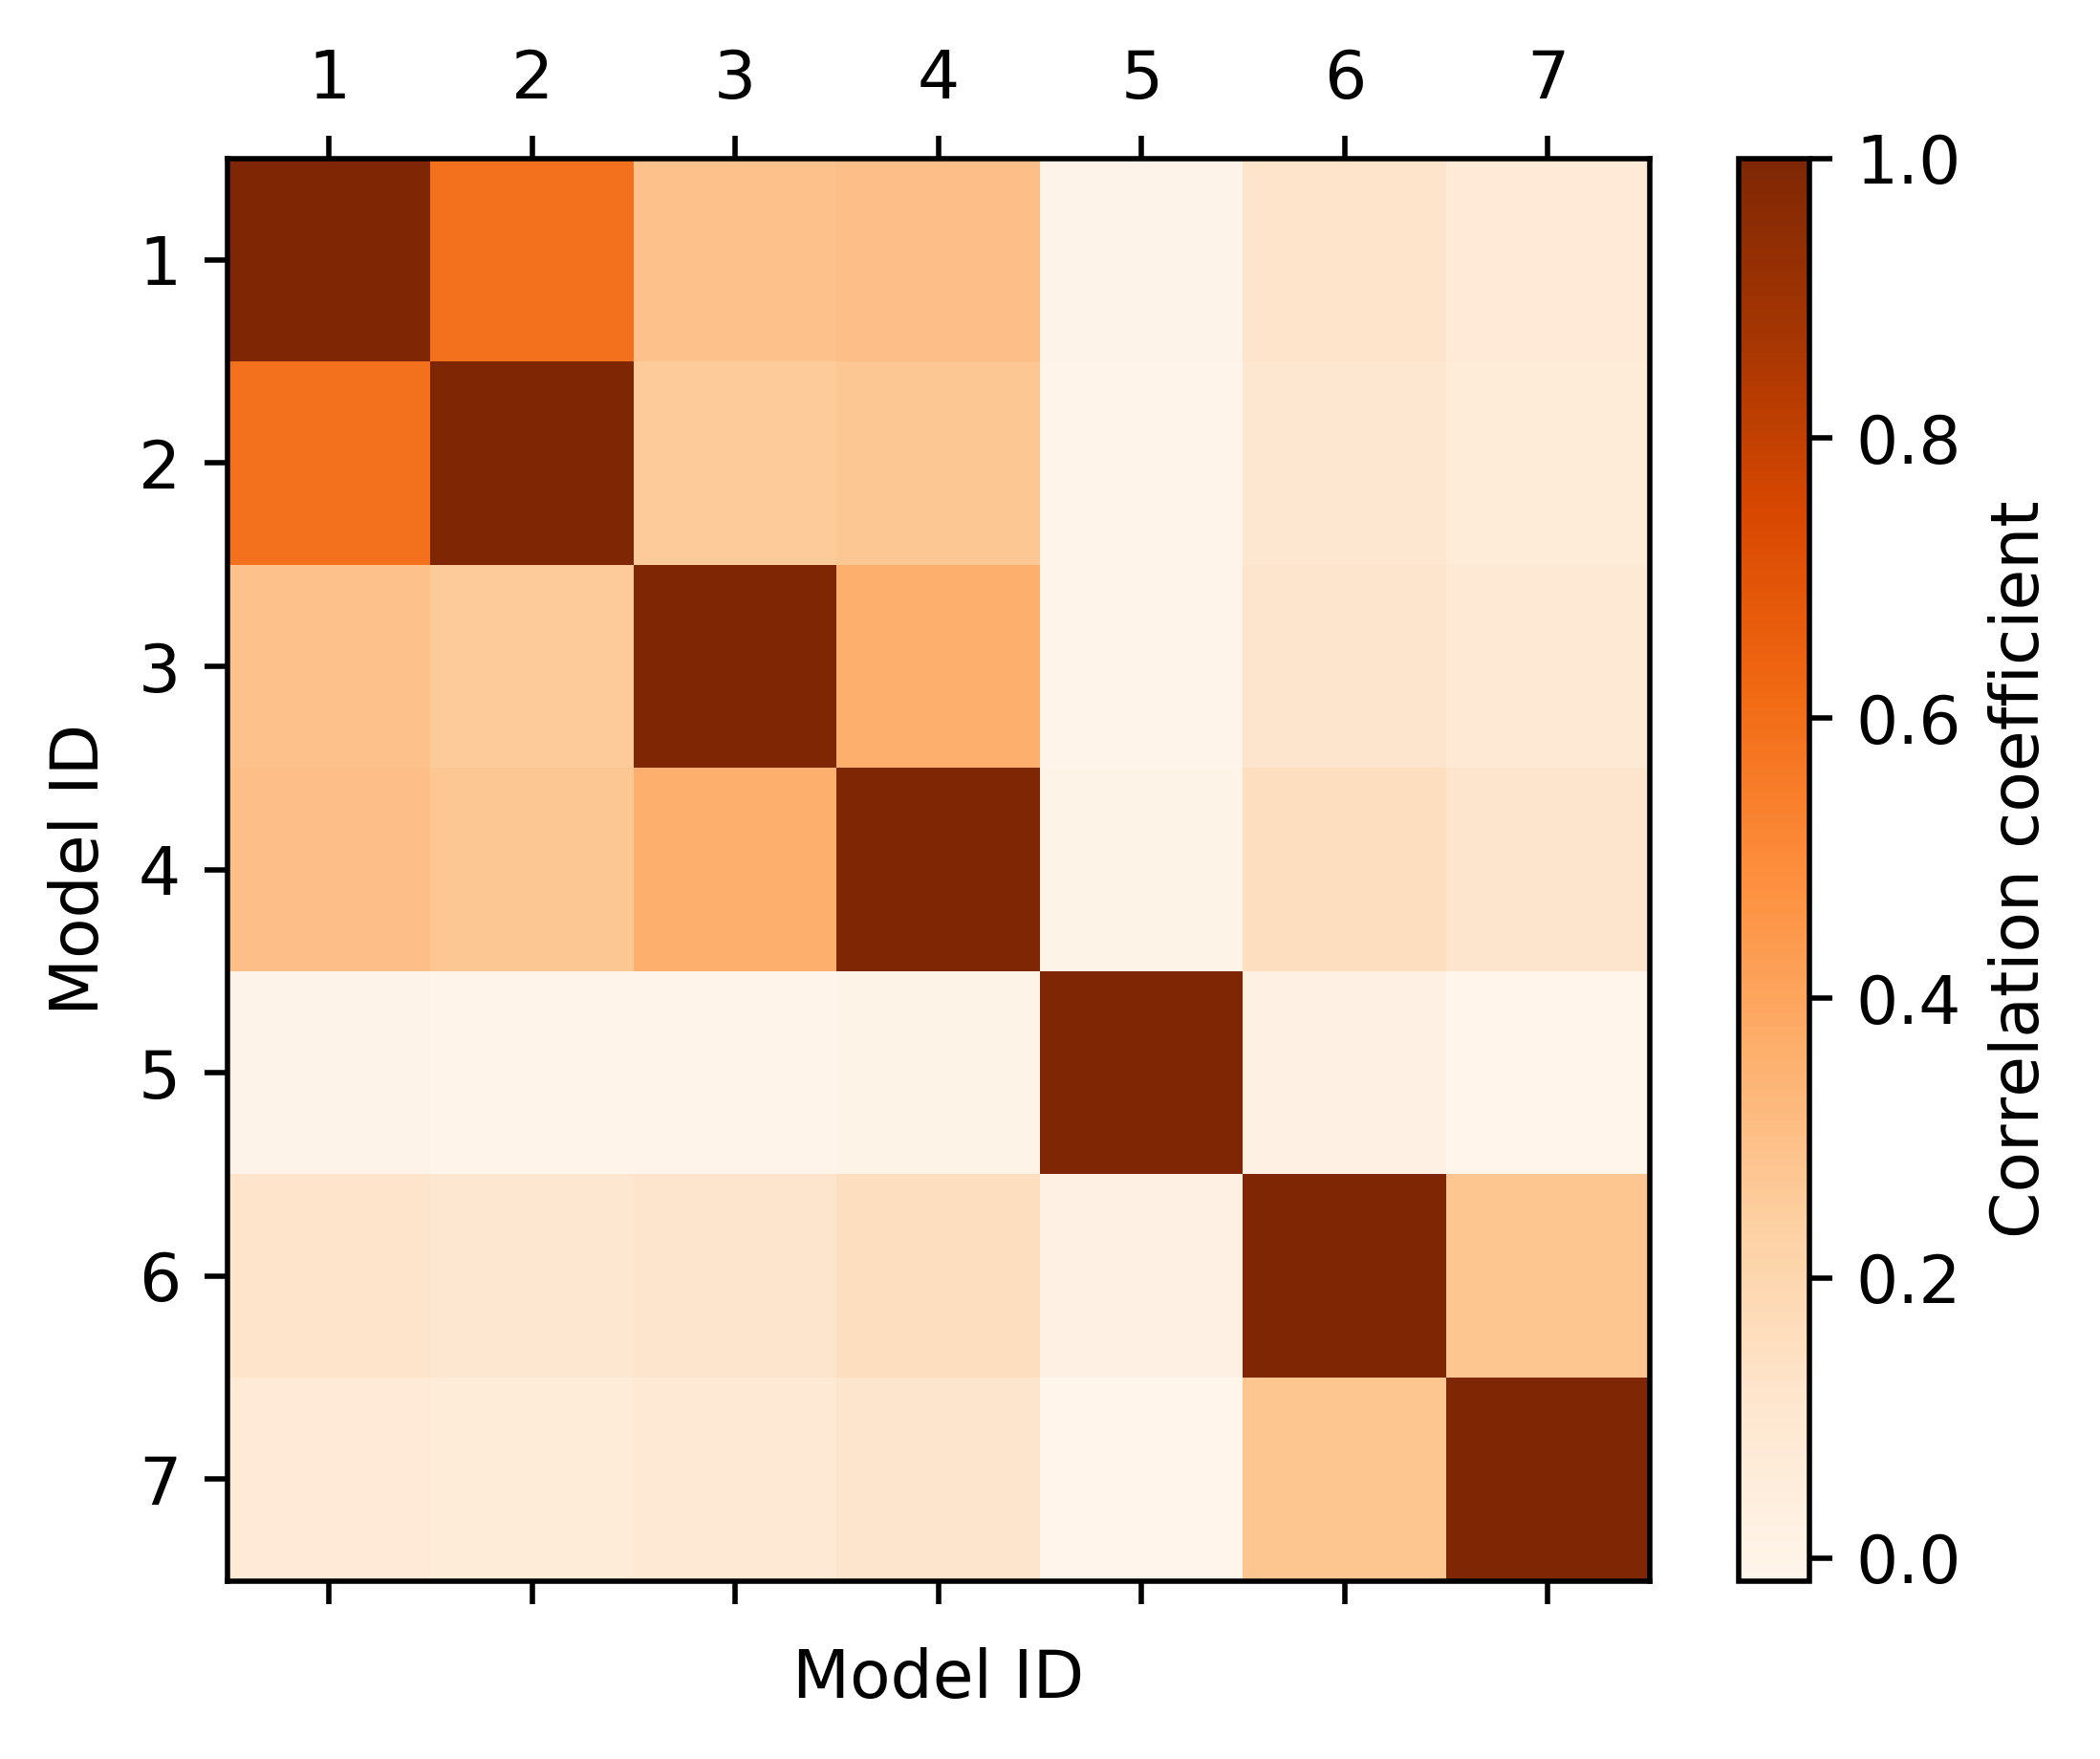
\includegraphics[width=0.3\textwidth]{fig/correlations.png}
	\caption{\textmd{Correlation matrix of our models using the test data set.}}
	\label{fig:correlation_matrix}
\end{figure}



\section{Evaluation}
We use \textit{precision} and \textit{recall} to evaluate our models. 
In practice, each article which produces a high amount of comments is more likely to bind resources of comment moderators and editors. Therefore, a high classification precision is important as well as a high recall to omit as few as possible.
Precision and recall are equally relevant and consequently, we use the harmonic mean, the $F_1$-score, of both metrics. As \textit{precision}, \textit{recall}, and the $F_1$-score are common metrics for binary classification problems, we are enabled to compare our results against existing approaches.

\subsection{Model Performances}
The overview of our results in \autoref{tbl:results_basic} depicts that all our models reach a significantly higher \textit{recall} than \textit{precision}.

\textit{Model 3} reaches the highest \textit{precision} with a value of $0.228$, and \textit{Model 7} the highest \textit{recall} with $0.917$. \textit{Model 4} is the best overall performing model with an $F_1$-score of $0.320$. 
%\textit{Model 1} to \textit{3} also performs relatively well with an $F_1$-scores of over $0.3$.

\textit{Model 1} and \textit{Model 2} process the same input. Despite the fact that the second model has approximately a third of the weights in its hidden layers, both models exhibit a similar performance for all three metrics.
We assume that the convolutional network can learn fewer features but has a much higher generalization potential through its shared weights.

\textit{Model 3} takes the first $50$ words of the article text as input. We discovered that using more or even all words has no positive effect on the model's predictions.

Compared to \textit{Model 1} and \textit{2} it reaches a worse \textit{recall} but a slightly higher \textit{precision} which leads to a similar $F_1$-score.
We suppose this occurs because of a similar context complexity which is provided by the headline and the first words of the article.

\textit{Model 4} achieves the best results. This seems surprising due to the low complexity of this feature but the relatively good results can be justified with the distribution of the categories within the GACC. 

\begin{figure}
	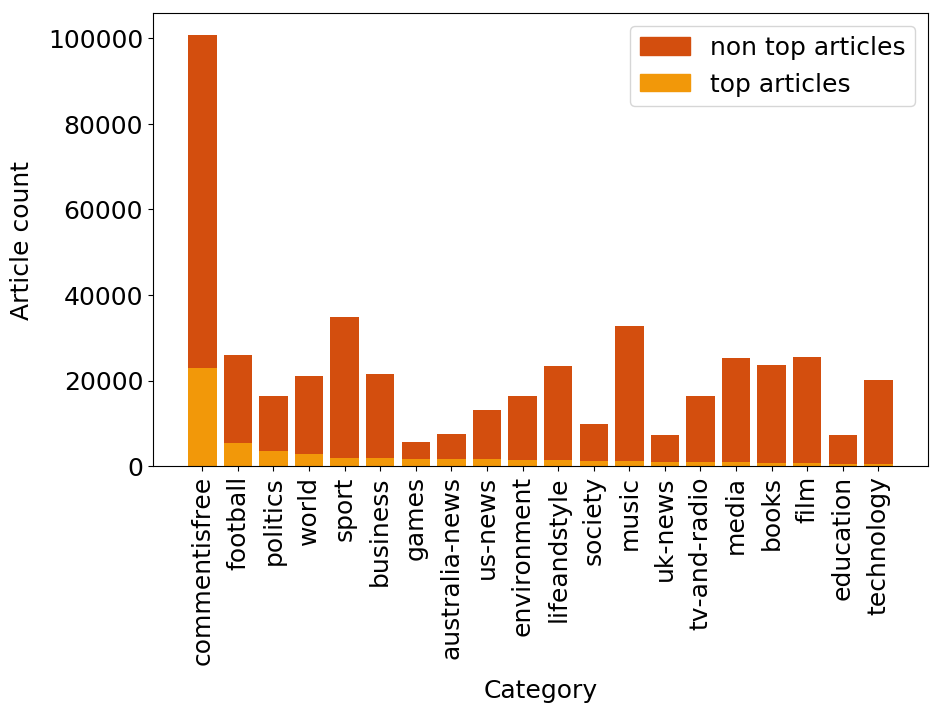
\includegraphics[width=0.45\textwidth]{fig/top_ten_category.png}
	\caption{\textmd{bla }}
	\label{fig:top_ten_category}
\end{figure}

Articles assigned to the most used category have a probability of $22.8\%$ to be a top article. Classifying just these articles as a top article already leads to an $F_1$-score of $0.292$. 
For instance, if we only classify articles within the four categories with the highest amount of top articles as a top article, we receive an $F_1$-score of $0.316$ which is almost as good as the result achieved by this model.

\textit{Model 5} is the worst performing model. Its precision of $0.100$ is just as good as a random prediction.

\begin{figure}
	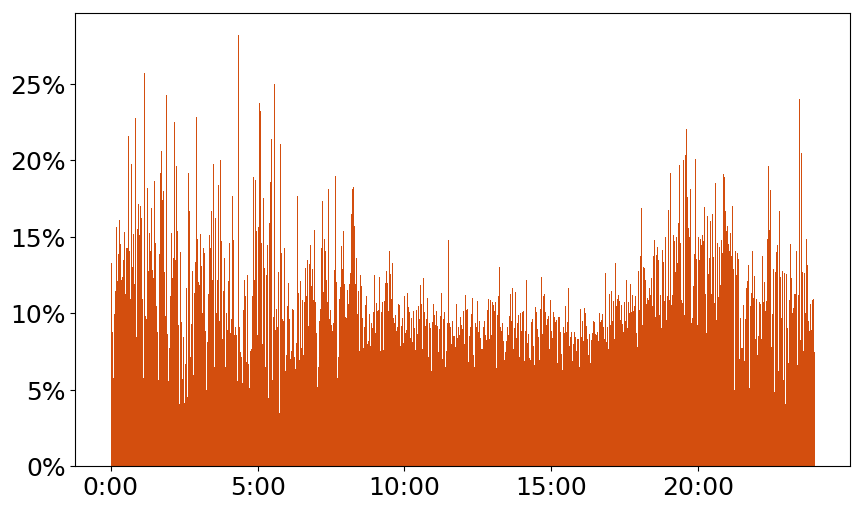
\includegraphics[width=0.45\textwidth]{fig/top_ten_time.png}
	\caption{\textmd{bla }}
	\label{fig:top_ten_time}
\end{figure}

One reason is that $19\%$ of all articles got released on full hours and might also be due to the fact that \textit{The Guardian} has an international readership spread over multiple time zones. Additionally, the day of the week has no significant effect on the weekly article performance. Therefore, this feature has almost no effect on the number of comments that an article receives. 

\textit{Model 6} had also a small but slightly better performance than \textit{Model 5}. 
Either the length of the headline or the length of the article text is feasible for an accurate prediction.

\textit{Model 7} processes just a single numeric value as input. For a good performance using the competitive score it would be necessary to be able to divide the values into distinct intervals that can be assigned to each class.
Unfortunately, the competitive score distribution of top articles is similar to the overall distribution of the competitive score.

% Table 3: Precision (P), recall (R), and F1-score of the baseline, all article and metadata features, annotations of comments shown on the first page, and all combined.
\begin{table}[h]
	\centering
	\caption{\textmd{Precision (P), recall (R), and $F_1$-score of all basic models.}}
	\label{tbl:results_basic}
	\vspace{-0.2cm}
	\begin{tabular}{cllccc}
		\toprule
		% \textbf{Features} &
		\specialcellbold{ID} &
		\specialcellbold{Input} &
		\specialcellbold{Type} &
		\specialcellbold{P} &
		\specialcellbold{R} &
		\specialcellbold{F$_1$} \\
		\midrule
		1 & headline & FC & .216 & .606  & .309  \\
		2 & headline & CNN & .221 & .603  & .314  \\
		3 & article & LSTM  & .228 & .493  & .302  \\
		4 & category & FC & .227 & .603  & .320  \\
		5 & time & FC  & .100 & .457  & .155  \\
		6 & text metrics & FC  & .133 & .738  & .222  \\
		7 & competitive score & FC & .112 & .917  & .197  \\
		\bottomrule
	\end{tabular}
\end{table}

\subsection{Combined Models}
As seen in \autoref{fig:correlation_matrix}, \textit{Model 1} and \textit{2} correlate the most with a value of $0.589$ which is due to processing the same input feature.
The correlation between \textit{Model 3} and both \textit{Model 1} and \textit{2} is also relatively high because the headline and the first $50$ words of the article provide a similar context.

We combine \textit{Model 2} with each other model because it exhibits the best results processing text input and has a low correlation to other models.
\textit{Model 5} which is correlating least with all other models has a very low $F_1$ score. Therefore, we exclude it from our consideration to combine it with every other model.

The combination of \textit{Model 2} with each \textit{Model 5}, \textit{6}, and \textit{7} doesn't have a better performance than \textit{Model 2} itself. 
Thus, we notice that the publishing time, text metrics, and competitive score are unqualified additional features for the headline text.

Combining each \textit{Model 3} and \textit{4} with \textit{Model 2} shows performance improvements. Consequently, we combine these models and receive our best \textit{precision} and $F_1$-score.

Compared to other approaches, our $F_1$-score is $37\%$ higher than the presented value from Tsagikas et al. \cite{tsagkias2009predicting} and $24\%$ smaller than the values from Ambroselli et al. \cite{ambroselli2018prediction}. 

Comparing our results one should keep in mind that our models used another dataset for their predictions.
The other results we are comparing against are achieved on a dataset containing German newspaper articles, and thus having a limited target audience and a limited range of topics.
Moreover the language suggests that the users behave more uniformly.
Therefore, the results are not necessarily comparable.

\begin{table}[]
\centering
\label{tbl:results_combined}
\caption{\textmd{Precision (P), recall (R), and F$_1$-score of all combined models}}
\vspace{-0.2cm}\begin{tabular}{cccc}
\toprule
% \textbf{Features} &
% \specialcellbold{Short description} &
\specialcellbold{Combination} &
\specialcellbold{P} &
\specialcellbold{R} &
\specialcellbold{F$_1$} \\
\midrule
2 3 & .224 & .645 & .323\\
2 4 & .245 & .627 & .342\\
2 5 & .227 & .581 & .317 \\
2 6 & .217 & .651 & .317\\
2 7 & .214 & .625 & .311\\
3 4 & .252 & .577 & .339\\
2 3 4 & .265 & .607 & .357\\
\bottomrule
\end{tabular}
\end{table}

\section{Conclusion}
In this paper, we studied the task of predicting the weekly top 10\% commented articles from the British newspaper \textit{The Guardian}. We tested different deep learning models in combination with different input features.

We reached our best results using a combination of a convolution layer for the embedded headlines, a LSTM layer for the embedded first words of the article and a FC layer for the category.

Using our approach on a different dataset we outperformed the baseline approach from Tsagkias et al. by $37\%$ and achieved a $8\%$ smaller $F_1$ as Ambroselli et al. for our prediction.



\bibliographystyle{acm}
\bibliography{sigproc} 

\end{document}
